%%%%%%%%%%%%%%%%%%%%%%%%%%%%%%%%%%%%%%%%%%%%%%%%%%%%%%%%
%                IAML 2020 Assignment 2                %
%                                                      %
%                                                      %
% Authors: Hiroshi Shimodaira and JinHong Lu           %
% Based on: Assignment 1 by Oisin Mac Aodha, and       %
%          Octave Mariotti                             %
% Using template from: Michael P. J. Camilleri and     %
% Traiko Dinev.                                        %
%                                                      %
% Based on the Cleese Assignment Template for Students %
% from http://www.LaTeXTemplates.com.                  %
%                                                      %
% Original Author: Vel (vel@LaTeXTemplates.com)        %
%                                                      %
% License:                                             %
% CC BY-NC-SA 3.0                                      %
% (http://creativecommons.org/licenses/by-nc-sa/3.0/)  %
%                                                      %
%%%%%%%%%%%%%%%%%%%%%%%%%%%%%%%%%%%%%%%%%%%%%%%%%%%%%%%%

%--------------------------------------------------------
%   IMPORTANT: Do not touch anything in this part
\documentclass[12pt]{article}
\input{style.tex}



% Options for Formatting Output

\global\setbool{clearon}{true} %
\global\setbool{authoron}{true} %
\ifbool{authoron}{\rhead{\small{\assignmentAuthorName}}\cfoot{\small{\assignmentAuthorName}}}{\rhead{}}



\newcommand{\assignmentQuestionName}{Question}
\newcommand{\assignmentTitle}{Assignment\ \#2}

\newcommand{\assignmentClass}{IAML -- INFR10069 (LEVEL 10)}

\newcommand{\assignmentWarning}{NO LATE SUBMISSIONS} % 
\newcommand{\assignmentDueDate}{Monday,\ November\ 23,\ 2020 @ 16:00}
%--------------------------------------------------------



%%%%%%%%%%%%%%%%%%%%%%%%%%%%%%%%%%%%%%%%%%%%%%%%%%%%%%%
%
% NOTE: YOU NEED TO ENTER YOUR STUDENT ID BELOW.
%
%%%%%%%%%%%%%%%%%%%%%%%%%%%%%%%%%%%%%%%%%%%%%%%%%%%%%%%% 
% --------------------------------------------------------
% IMPORTANT: Specify your Student ID below. You will need to uncomment the line, else compilation will fail. Make sure to specify your student ID correctly, otherwise we may not be able to identify your work and you will be marked as missing.
\newcommand{\assignmentAuthorName}{s1864480}
%--------------------------------------------------------



\begin{document}


%%%%%%%%%%%%%%%%%%%%%%%%%%%%%%%%%%%%%%%%%%%%%%%%%%%%%%%%%%%%%%%%%%%%%%%%%%%%%%
%============================================================================%
%%%%%%%%%%%%%%%%%%%%%%%%%%%%%%%%%%%%%%%%%%%%%%%%%%%%%%%%%%%%%%%%%%%%%%%%%%%%%%
\clearpage
%
% Question 1
%

\begin{question}{(30 total points) Image data analysis with PCA}

  
  \questiontext{In this question we employ PCA to analyse image data}
  

  
  \medskip

   %==============================
   % Q1.1
  \begin{subquestion}{(3 points)
      Once you have applied the normalisation from Step 1 to Step 4 above,
      report the values of the first 4 elements for the first training
      sample in \texttt{Xtrn\_nm},
      i.e. \texttt{Xtrn\_nm[0,:]} and the last training sample,
      i.e. \texttt{Xtrn\_nm[-1,:]}.
    } \label{Q1.1}
    

      \begin{answerbox}{10em}
         The first 4 elements of the first and the last training sample are:
         $$[-0.    , -0.    , -0.0001, -0.0004]$$
      \end{answerbox}
  


   \end{subquestion}
   %
   % ==============================
   % 
   % Q1.2
   \begin{subquestion}{(4 points)
      Using {\tt Xtrn} and Euclidean distance
      measure, for each class,
      find the two closest samples and two furthest
      samples of that class to the mean vector of the class.
    }  \label{Q1.2}




  \begin{answerbox}{52em}
    \begin{center}
        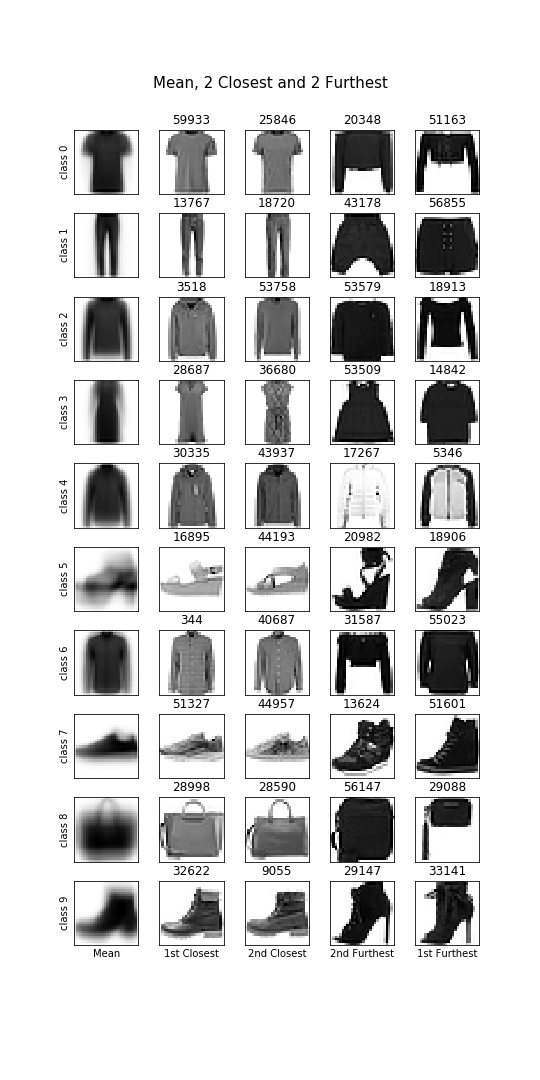
\includegraphics[width=0.75\textwidth, height=39em]{results/1_2.png}
    \end{center}
    The mean image of each data class shows us the shape and general outline/boundary of all the images in it. We can visually see the significantly large differences between the closest and furthest images to the mean. The closest images retain the shape and outline of their corresponding mean class which was expected as they are the nearest samples to it. In these samples the "dark" and "light" areas match the mean images "dark" and "light" areas. Whereas when we look at the furthest samples we can clearly see that they have a different boundary/outline, general shape, and big and sometimes significant differences in their "dark"/"light" areas. 
  \end{answerbox}



   \end{subquestion}

   % 
   % Q1.3
   \begin{subquestion}{(3 points)
       Apply Principal Component Analysis (PCA) to the data of {\tt
         Xtrn\_nm} using
       \href{https://scikit-learn.org/0.19/modules/generated/sklearn.decomposition.PCA.html}{sklearn.decomposition.PCA},
       and report the variances of projected data for the first five principal
       components in a table. Note that you should use {\tt Xtrn\_nm} instead of {\tt Xtrn}.} 
    \label{Q1.pca.variance}
     


    \begin{answerbox}{15em}
        \centering
        \begin{tabular}{|c|l|}
            \hline
            \multicolumn{1}{|l|}{\textbf{Principal Component (PC)}} & \textbf{Variance} \\ \hline
            PC1                                            & 19.8098  \\ \hline
            PC2                                            & 12.1122  \\ \hline
            PC3                                            & 4.1062   \\ \hline
            PC4                                            & 3.3818   \\ \hline
            PC5                                            & 2.624    \\ \hline
        \end{tabular}
    \end{answerbox}
    


   \end{subquestion}

   %==============================
   % Q1.4
   \begin{subquestion}{(3 points)
       Plot a graph of the cumulative explained variance ratio as a
       function of the number of principal components, $K$, where $1
       \le K \le 784$.
       Discuss the result briefly.
       } \label{Q1.plot.pca.variance}
   

      \begin{answerbox}{30em}
        \begin{center}
            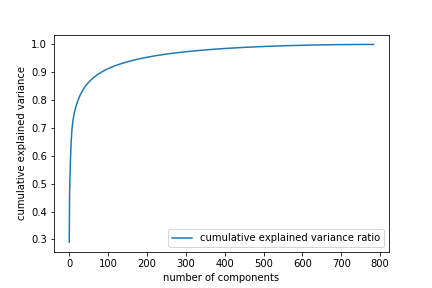
\includegraphics[width=0.72\textwidth]{results/1_4.png}
        \end{center}
        This curve shows how much of the total, 784-dimensional variance is contained within the first $N$ components. The curve is extremely steep in the beginning and quickly plateaus. Here we can see that approximately first $20$ components contain $80\%$ of the variance, the first $100$ components contain approximately $90\%$ of the variance, and we would need around $500$ components to describe close to $100\%$ of the variance. This knowledge allows us to work with and explore the dataset more easily, as we can project our $784$ to much smaller dimensions, for eg. $100$ without losing much information. 
      \end{answerbox}
  


   \end{subquestion}

   %==============================
   % Q1.5
   \begin{subquestion}{(4 points)
      Display the images of the first 10 principal components in
      a 2-by-5 grid, putting the image of 1st principal component on
      the top left corner, followed by the one of 2nd component to the right.
      Discuss your findings briefly.
     } \label{Q1.disp.pca}
   

      \begin{answerbox}{35em}
         \begin{center}
            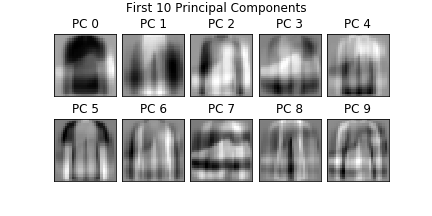
\includegraphics[width=0.9\textwidth]{results/1_5.png}
        \end{center}
        As seen in the previous question, the principal components upto $20$ express most of the variance in the dataset which is necessary to capture the features/characteristics of the dataset and differentiate between classes. It has been discussed in the lectures, that really dark and light/bright areas in the plot correspond to the dominating factors with which we differentiate classes. The gray and dull areas don't affect the differentiation a lot. In this plot we can see most of the subplots have clear images of some upper-body wear like shirts, t-shirts, coats, pullovers or footwear like sneakers, sneakers and boots. This is again something we would expect, as considering the classes of the dataset ($\frac{4}{10}$ upper-body wear, $\frac{3}{10}$ are footwear) these are the shapes/patterns which contain most of the variance. In some of the subplots we can vaguely see the outline of other classes like dresses as well.
    \end{answerbox}
  


   \end{subquestion}

   %==============================
   % Q1.6
   \begin{subquestion}{(5 points)
       Using \texttt{Xtrn\_nm}, 
       for each class and for each number of principal components $K =
       5, 20, 50, 200$, apply dimensionality reduction with PCA to the
       first sample in the class, reconstruct the sample from the
       dimensionality-reduced sample, and 
       report the Root Mean Square Error (RMSE) between the
       original sample in {\tt Xtrn\_nm} and reconstructed one.
     } \label{Q1.6}

     

      \begin{answerbox}{25em}
         \centering
        \begin{tabular}{|c|l|l|l|l|l|l|l|l|}
            \hline
            \textbf{Class} & \textbf{K} & \textbf{RSME} & \textbf{K} & \textbf{RSME} & \textbf{K} & \textbf{RSME} & \textbf{K} & \textbf{RSME}   \\ \hline
            0     & 5 & 0.2561 & 20 & 0.1501 & 50 & 0.127 & 200 & 0.0619 \\ \hline
            1     & 5 & 0.198 & 20 & 0.1404 & 50 & 0.0952 & 200 & 0.0361 \\ \hline
            2     & 5 & 0.1987 & 20 & 0.1455 & 50 & 0.1224 & 200 & 0.0798 \\ \hline
            3     & 5 & 0.1457 & 20 & 0.1075 & 50 & 0.0838 & 200 & 0.0561 \\ \hline
            4     & 5 & 0.1182 & 20 & 0.1026 & 50 & 0.087 & 200 & 0.0466 \\ \hline
            5     & 5 & 0.1811 & 20 & 0.1586 & 50 & 0.1431 & 200 & 0.0898 \\ \hline
            6     & 5 & 0.1295 & 20 & 0.0963 & 50 & 0.0725 & 200 & 0.0446 \\ \hline
            7     & 5 & 0.1656 & 20 & 0.1272 & 50 & 0.1059 & 200 & 0.0614 \\ \hline
            8     & 5 & 0.2234 & 20 & 0.1449 & 50 & 0.1233 & 200 & 0.093 \\ \hline
            9     & 5 & 0.1835 & 20 & 0.1513 & 50 & 0.1218 & 200 & 0.0716 \\ \hline
        \end{tabular}
      \end{answerbox}
  


   \end{subquestion}
   
   %==============================
   % Q1.7
   \begin{subquestion}{(4 points)
       Display the image for each of the reconstructed samples in
       a 10-by-4 grid, where each row corresponds to a class and
       each row column corresponds to a value of $K=5, \; 20, \; 50, \; 200$.
     } \label{Q1.7}


   

      \begin{answerbox}{52em}
         \begin{center}
             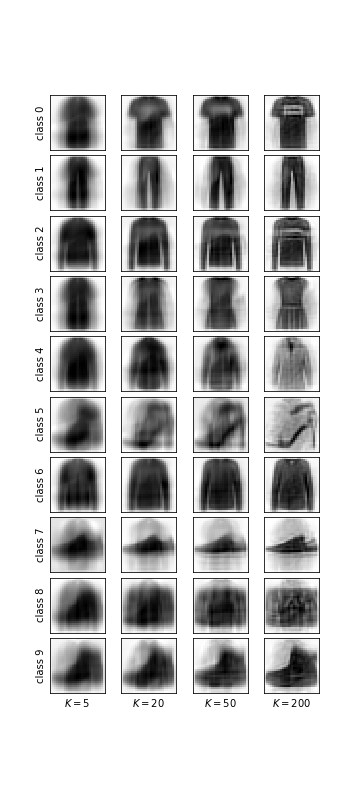
\includegraphics[width=0.75\textwidth, height=37em]{results/1_7.png}
         \end{center}
         We can see in the plot that more the number of principal components, more is the clarity and definition of the image. On the other hand we can also observe that even when using low values of $K$ like $5$ or $20$, we are still able to capture many of the characteristics. This is logical as we have seen in previous questions as how by increasing the number of components we can capture a lot more variance in the data but the first few components alone can explain most of the variance in the dataset. From the previous question we can also say that the RSME value decreases as the number of component increases and we can see how our images are more sharper and truer to their class.
      \end{answerbox}
  


   \end{subquestion}
   %==============================
   %
   %==============================
   % Q1.8
   \begin{subquestion}{(4 points)
       Plot all the training samples (\texttt{Xtrn\_nm}) on the
       two-dimensional PCA plane you obtained in \refQ{Q1.pca.variance}, where each sample is
       represented as a small point with a colour specific to the class of
       the sample.  Use the 'coolwarm' colormap for plotting.
     } \label{Q1.8}


   

      \begin{answerbox}{40em}
         \begin{center}
             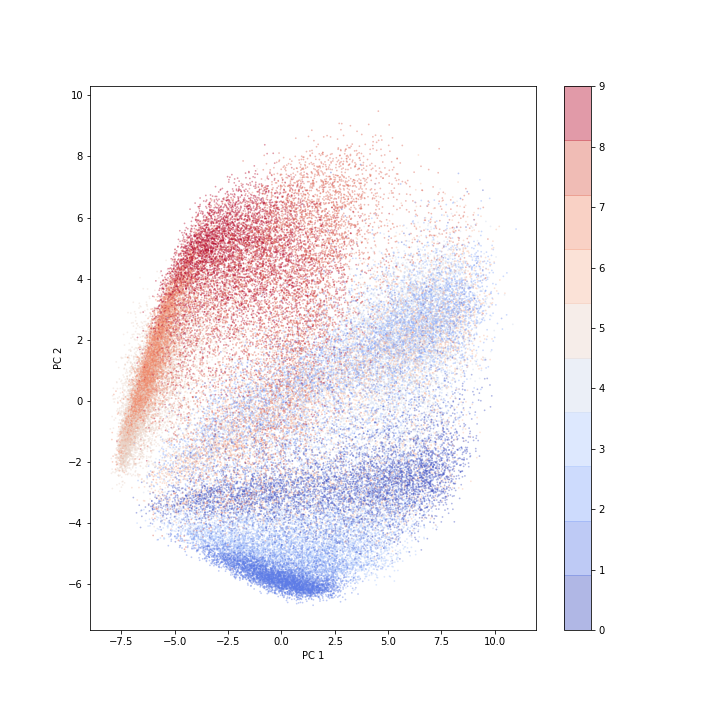
\includegraphics[width=0.75\textwidth]{results/1_8.png}
         \end{center}
         The data is quite clearly not linearly separable, but from this scatter plot of the projection of training samples see can see that most samples of each class are clustered together. We can also clearly identify a few more characteristic of the plot; similar classes are clustered near each other, i.e. upper body wear is scattered downwards while footwear classes are projected upwards of the graph.
      \end{answerbox}
  


   \end{subquestion}
   %
   %==============================
   

\end{question}
%%%%%%%%%%%%%%%%%%%%%%%%%%%%%%%%%%%%%%%%%%%%%%%%%%%%%%%%%%%%%%%%%%%%%%%%%%%%%%
%============================================================================%
%%%%%%%%%%%%%%%%%%%%%%%%%%%%%%%%%%%%%%%%%%%%%%%%%%%%%%%%%%%%%%%%%%%%%%%%%%%%%%
\clearpage
%
% Question 2
%
\begin{question}{(25 total points) Logistic regression and SVM}

  \questiontext{In this question we will explore 
    classification of image data with logistic regression and support
    vector machines (SVM) and visualisation 
    of decision regions.
  }
  


  \medskip
   %==============================
   % Q2.1
   \begin{subquestion}{(3 points)
       Carry out a classification experiment with
       \href{https://scikit-learn.org/0.19/modules/generated/sklearn.linear\_model.LogisticRegression.html}{multinomial logistic regression},
       and report the classification accuracy and confusion matrix (in
       numbers rather than in graphical representation such as heatmap)
       for the test set.
     } \label{Q2.1}


   

      \begin{answerbox}{30em}
        
        \textbf{Table of confusion matrix for the test set}
        \medskip
        \centering
        \small
        \begin{tabular}{@{}lllllllllll@{}}
        \toprule
             & 0 & 1 & 2 & 3 & 4 & 5 & 6 & 7 & 8 & 9 \\ \midrule
            0 & 819 & 3 & 15 & 50 & 7 & 4 & 89 & 1 & 12 & 0 \\ 
            1 & 5 & 953 & 4 & 27 & 5 & 0 & 3 & 1 & 2 & 0 \\ 
            2 & 27 & 4 & 731 & 11 & 133 & 0 & 82 & 2 & 9 & 1 \\ 
            3 & 31 & 15 & 14 & 866 & 33 & 0 & 37 & 0 & 4 & 0 \\ 
            4 & 0 & 3 & 115 & 38 & 760 & 2 & 72 & 0 & 10 & 0 \\ 
            5 & 2 & 0 & 0 & 1 & 0 & 911 & 0 & 56 & 10 & 20 \\ 
            6 & 147 & 3 & 128 & 46 & 108 & 0 & 539 & 0 & 28 & 1 \\ 
            7 & 0 & 0 & 0 & 0 & 0 & 32 & 0 & 936 & 1 & 31 \\ 
            8 & 7 & 1 & 6 & 11 & 3 & 7 & 15 & 5 & 945 & 0 \\ 
            9 & 0 & 0 & 0 & 1 & 0 & 15 & 1 & 42 & 0 & 941 \\ \bottomrule 
        \end{tabular}

        \medskip
        \noindent
        \textbf{Classification Accuracy:}
        $$84.01\%$$
      \end{answerbox}
  


   \end{subquestion}
   %
   % ==============================
   %
   %==============================
   % Q2.2
   \begin{subquestion}{(3 points)
       Carry out a classification experiment with
       \href{https://scikit-learn.org/0.19/modules/generated/sklearn.svm.SVC.html}{SVM classifiers}, and report the
       mean accuracy and confusion matrix (in numbers) for the test
       set.
     } \label{Q2.2}


   

      \begin{answerbox}{30em}
        \textbf{Table of confusion matrix for the test set}
        \bigskip
        \small
        \centering
        \begin{tabular}{@{}lllllllllll@{}}
        \toprule
             & 0 & 1 & 2 & 3 & 4 & 5 & 6 & 7 & 8 & 9 \\ \midrule
            0 & 845 & 2 & 8 & 51 & 4 & 4 & 72 & 0 & 14 & 0 \\ 
            1 & 4 & 951 & 7 & 31 & 5 & 0 & 1 & 0 & 1 & 0 \\ 
            2 & 15 & 2 & 748 & 11 & 137 & 0 & 79 & 0 & 8 & 0 \\ 
            3 & 32 & 6 & 12 & 881 & 26 & 0 & 40 & 0 & 3 & 0 \\ 
            4 & 1 & 0 & 98 & 36 & 775 & 0 & 86 & 0 & 4 & 0 \\ 
            5 & 0 & 0 & 0 & 1 & 0 & 914 & 0 & 57 & 2 & 26 \\ 
            6 & 185 & 1 & 122 & 39 & 95 & 0 & 533 & 0 & 25 & 0 \\ 
            7 & 0 & 0 & 0 & 0 & 0 & 34 & 0 & 925 & 0 & 41 \\ 
            8 & 3 & 1 & 8 & 5 & 2 & 4 & 13 & 4 & 959 & 1 \\ 
            9 & 0 & 0 & 0 & 0 & 0 & 22 & 0 & 47 & 1 & 930 \\ \bottomrule 
        \end{tabular}
        
        \medskip
        \noindent
        \textbf{Classification Accuracy:}
        $$84.61\%$$

      \end{answerbox}
  


   \end{subquestion}
   %
   % ==============================
   %
   %==============================
   % Q2.3
   \begin{subquestion}{(6 points)
       We now want to visualise the decision regions for the logistic
       regression classifier we trained in \refQ{Q2.1}.
     } \label{Q2.3}


   

      \begin{answerbox}{35em}
         \begin{center}
             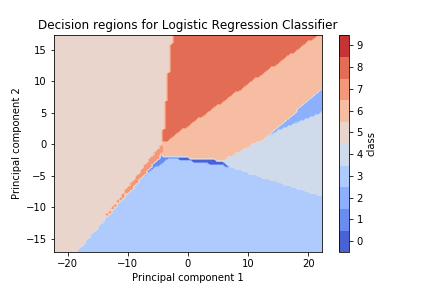
\includegraphics[width=\textwidth]{results/2_3.png}
         \end{center}
      \end{answerbox}
  


   \end{subquestion}
   %
   % ==============================
   %
   %==============================
   % Q2.4
   \begin{subquestion}{(4 points)
       Using the same method as the one above, plot the decision regions for
       the SVM classifier you trained in \refQ{Q2.2}.
       Comparing the result with that you obtained in \refQ{Q2.3}, discuss your
       findings briefly.
     } \label{Q2.4}
   

      \begin{answerbox}{35em}
         \begin{center}
               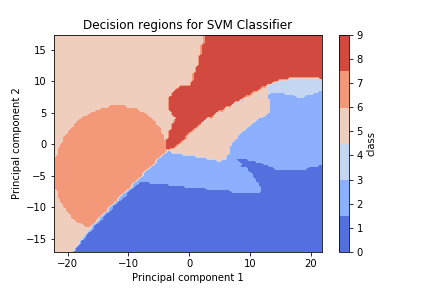
\includegraphics[width=0.9\textwidth]{results/2_4.png}
         \end{center}
         TODO
      \end{answerbox}
  


   \end{subquestion}
   %
   % ==============================
   %

   %==============================
   % Q2.5
   \begin{subquestion}{(6 points)
       We used default parameters for the SVM in \refQ{Q2.2}.
       We now want to tune the parameters by using cross-validation.
       To reduce the time for experiments, you pick up the first 1000
       training samples from each class to create \texttt{Xsmall}, so that \texttt{Xsmall}
       contains 10,000 samples in total. Accordingly, you create
       labels, \texttt{Ysmall}.
     } \label{Q2.5}


   

      \begin{answerbox}{30em}
        \begin{center}
            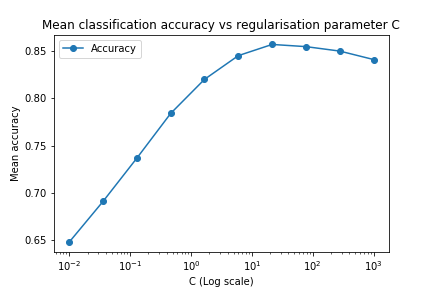
\includegraphics[width=0.9\textwidth]{results/2_5.png}    
        \end{center}
        \textbf{Highest Obtained Mean Accuracy: } $85.65\%$
        \newline
        \textbf{Value of C: } $21.544$
      \end{answerbox}
  


   \end{subquestion}
   %
   % ==============================
   %
   %==============================
   % Q2.6
   \begin{subquestion}{(3 points)
       Train the SVM classifier on the whole training set by using the
       optimal value of $C$ you found in \refQ{Q2.5}. 
     } \label{Q2.6}


       

      \begin{answerbox}{10em}
        \textbf{Accuracy of the improved SVM classifier:}
        \medskip
        \begin{center}
            \begin{tabular}{c|c}
            \toprule
              Train & Test \\ \hline
              $90.842\%$ & $87.65\%$ \\
            \bottomrule
         \end{tabular}
        \end{center}
      \end{answerbox}
  


   \end{subquestion}
   %
   % ==============================
   %
%
%

\end{question}
%%%%%%%%%%%%%%%%%%%%%%%%%%%%%%%%%%%%%%%%%%%%%%%%%%%%%%%%%%%%%%%%%%%%%%%%%%%%%%
%============================================================================%
%%%%%%%%%%%%%%%%%%%%%%%%%%%%%%%%%%%%%%%%%%%%%%%%%%%%%%%%%%%%%%%%%%%%%%%%%%%%%%
\clearpage
%
% Question 3
%

\begin{question}{(20 total points) Clustering and Gaussian Mixture Models}  


  \questiontext{In this question we will explore K-means clustering,
    hierarchical clustering, and GMMs.
  }
  


  \medskip
   %==============================
   % Q3.1
   \begin{subquestion}{(3 points)
       Apply k-means clustering on {\tt Xtrn} for $k = 22$, where we use
       \href{https://scikit-learn.org/0.19/modules/generated/sklearn.cluster.KMeans.html}{sklearn.cluster.KMeans}
       with the parameters {\tt n\_clusters=22} and {\tt random\_state=1}.
       Report the sum of squared distances of samples to their closest
       cluster centre, and the number of samples for each cluster.
     } \label{Q3.1}
   

      \begin{answerbox}{35em}
        Sum of squared distances of samples to their closest cluster centre = $38185.817$
         \begin{center}
            \begin{tabular}{|c|c|}
                \toprule
                Cluster & Num of Samples \\ \hline
                0 & 1018 \\
                1 & 1125 \\
                2 & 1191 \\
                3 & 890 \\
                4 & 1162 \\
                5 & 1332 \\
                6 & 839 \\
                7 & 623 \\
                8 & 1400 \\
                9 & 838 \\
                10 & 659 \\
                11 & 1276 \\
                12 & 121 \\
                13 & 152 \\
                14 & 950 \\
                15 & 1971 \\
                16 & 1251 \\
                17 & 845 \\
                18 & 896 \\
                19 & 930 \\
                20 & 1065 \\
                21 & 1466 \\
                \bottomrule
            \end{tabular}    
         \end{center}
         
      \end{answerbox}
  


   \end{subquestion}
   %
   % ==============================
   %
   %==============================
   % Q3.2
   \begin{subquestion}{(3 points)
       Using the training set only,
       calculate the mean vector for each language, and plot the mean
       vectors of all the 22 languages on a 2D-PCA plane, where you
       apply PCA on the set of 22 mean vectors without applying
       standardisation.  
       On the same figure, plot the cluster centres obtained in \refQ{Q3.1}.
     } \label{Q3.2}

   

      \begin{answerbox}{35em}
         \begin{center}
             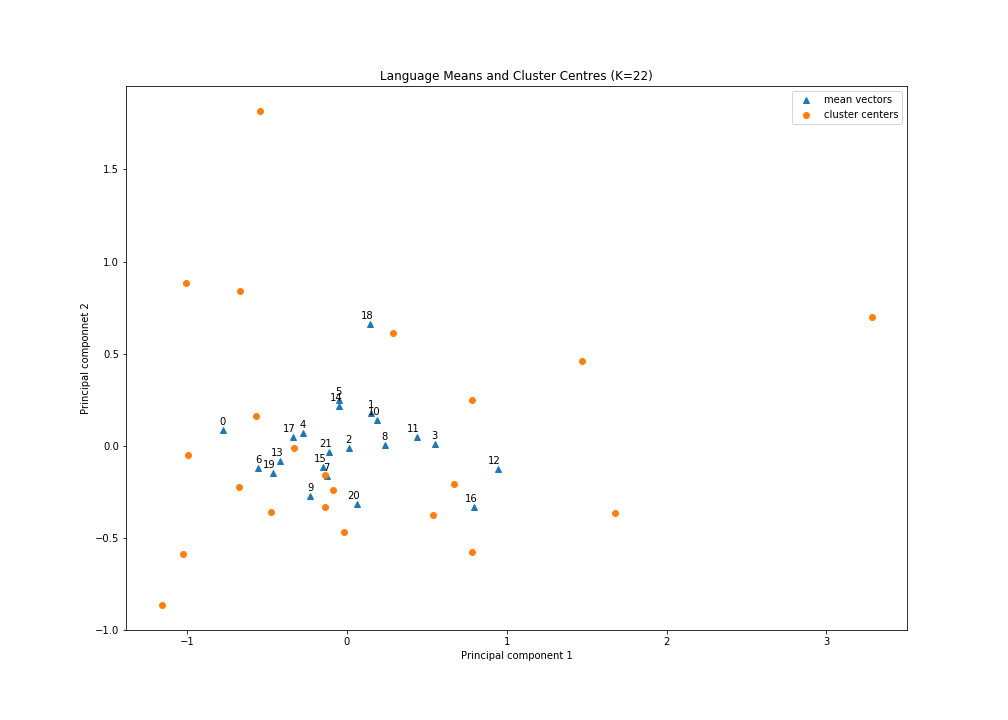
\includegraphics[width=\textwidth]{results/3_2.png}
         \end{center}
      \end{answerbox}
  


   \end{subquestion}
   %
   % ==============================
   %
   %==============================
   % Q3.3
   \begin{subquestion}{(3 points)
       We now apply hierarchical clustering on the training data set
       to see if there are any structures in the spoken languages.
     } \label{Q3.3}


     

      \begin{answerbox}{35em}
        \begin{center}
            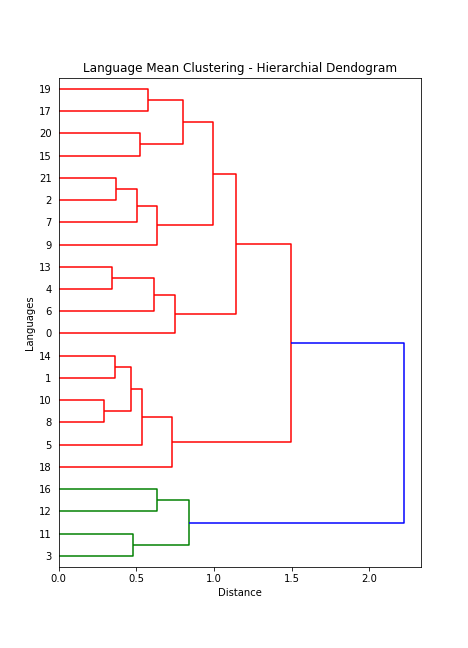
\includegraphics[width=0.6\textwidth]{results/3_3.png}
        \end{center}
      \end{answerbox}
  


   \end{subquestion}
   %
   % ==============================
   %
   %==============================
   % Q3.4
   \begin{subquestion}{(5 points)
       We here extend the hierarchical clustering done in \refQ{Q3.3} by
       using multiple samples from each language.
     } \label{Q3.4}


   

      \begin{answerbox}{50em}
         \begin{center}
            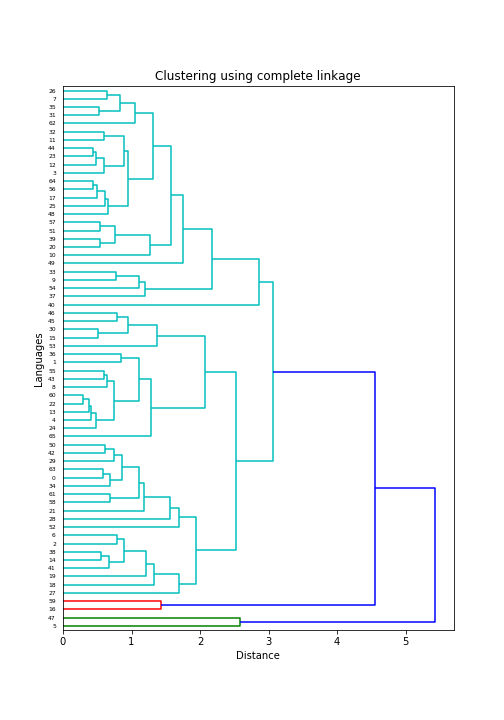
\includegraphics[width=0.81\textwidth, height=16em]{results/3_4_complete.png}\vfill
            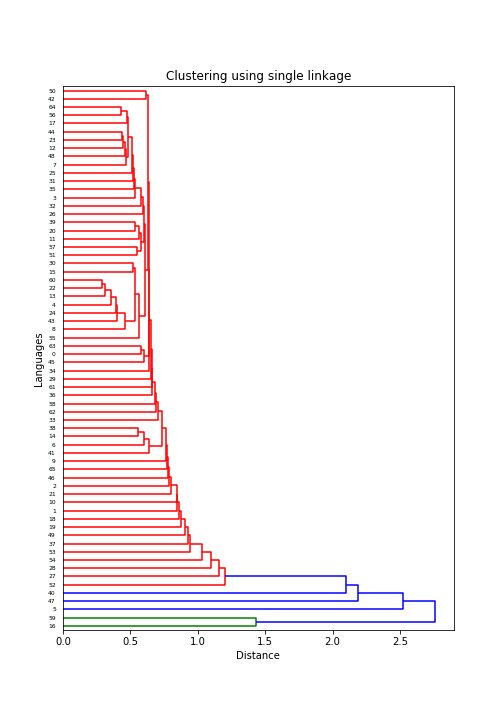
\includegraphics[width=0.81\textwidth, height=16em]{results/3_4_single.png}\vfill
            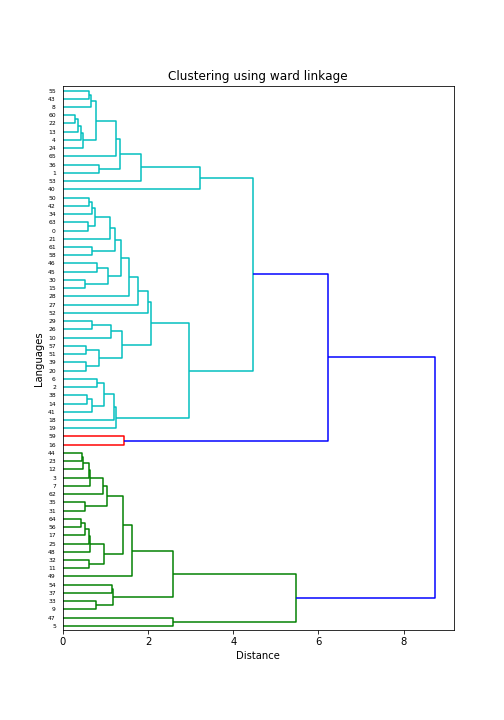
\includegraphics[width=0.81\textwidth, height=16em]{results/3_4_ward.png}

         \end{center}
      \end{answerbox}
  


   \end{subquestion}
   %
   % ==============================
   %
   %==============================
   % Q3.5
   \begin{subquestion}{(6 points)
       We now consider Gaussian mixture model (GMM), whose
       probability distribution function (pdf) is given as
       a linear combination of Gaussian or normal distributions, i.e.,
     } \label{Q3.5}




      \begin{answerbox}{30em}
         \begin{center}
             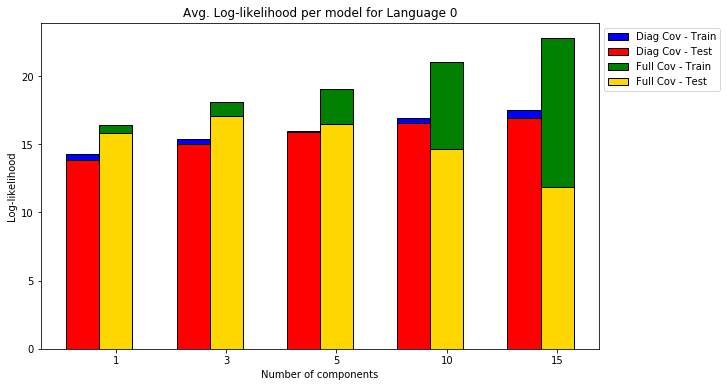
\includegraphics[width=\textwidth]{results/3_5.png}
         \end{center}
      \end{answerbox}
  


   \end{subquestion}
   %
   %==============================

   % ==============================
   
\end{question}
\end{document}
